
\section{Notizen, die ich später noch gebrauchen könnte}
............................................................

regelt horizontale Integration aus Produktionssicht und vertikale Integration des Assets aus IT-Sicht. Dabei werden die Daten über den gesamten Lebenszyklus von Prduktionsgegenständen/Komponenten gesammelt. Von typ zu Instanz.
Die Vertikale Sicht ist der Fokus dieser Arbeit.  Die vom Asset erzeugten Daten werden mit einer standardisierten Kommunikation (OPC UA) über den Kommunikationslayer an den funktional Player weitergegeben. Miaaaaau

Die senkrechte Achse bezieht sich auf die vertikale Integration des realen Produktionsgegenstandes (Asset), dessen virtuelle Repräsentation über die Integrantionsschicht erstellt wird. Zu den Assets werden sowohl alle in der Anlage verbauten physischen Komponenten als auch andere Vermögensgegenstände wie Software oder Patente, aber auch Menschen, gezählt \citep{Adolphs2017}.
 Über die Kommunikationsschicht

 Durch die horizontale Integration können technische, administrative sowie kommerzielle Daten über die gesamte Wertschöpfungskette hinweg konsisten gehalten werden.


Grundlage für neue Produkte zur Cloud-basierten Kommunikation


Die beiden horizontalen Achsen beschreiben Anforderungen und Voraussetzzungen für eine Industrie-4.0-Architektur aus Produktionssicht. In dieser Arbeit wird der Fokus auf die IT-Sicht gelegt. Daher wird die verikale Integration des Asstets genauer erläutert.
Auf vertikaler Achse wird das Asset, also der Gegenstand behandelt. Ziel ist die komplette Integration und die Vernezung der Produktionssysteme in Echtzeit. Asset-Layer, Integration-Layer, Commucation Layer-Standardisierte Kommunikation, Information Layer Datenhaltung, Functional



\begin{figure}[h]
  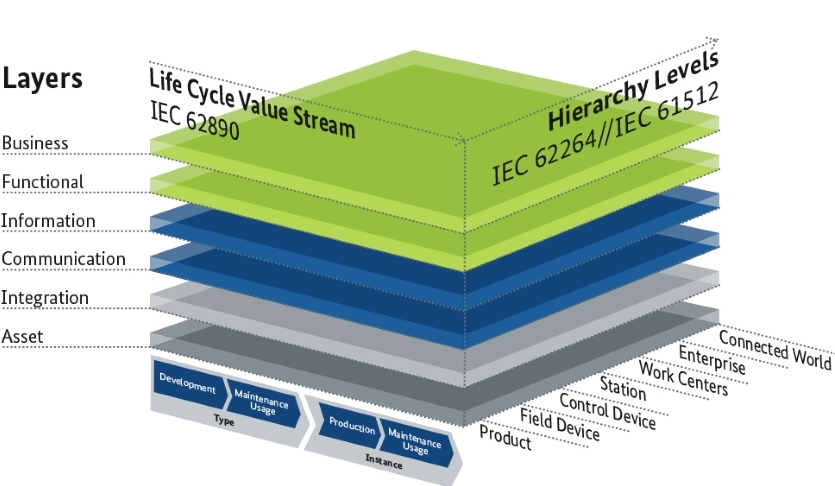
\includegraphics[width=1.0\linewidth]{RAMI.png}
  \caption[Das Referenzarchitekturmodell Industrie 4.0]{Das Referenzarchitekturmodell Industrie 4.0 \citep{BITKOM2015}}
  \label{fig:rami}
\end{figure}

\paragraph{Die Industrie-4.0-Komponente}


\begin{itemize}
  \item Bitkom bzw. Plattform Industrie 4.0 stellt Referenzarchitektur
  \item RAMI bietet die Möglichkeit, Industrie 4.0 UseCases zu verorten, um die für den jeweiligen use case notwendigen Normen und Standards zu identfizieren
  \item horizontale Integration über Wertschöpfungsnetzwerke: Lieferanten, Unternehmen, Produzenten
  \item Durchgängigkeit des Engineerings: Systems Engineering, Modellierung, Simulation
  \item vertikale Integration und vernetzte Pproduktionssysteme mit Echtzeitanforderung
  \item neue soziale Infrastrukturen der Arbeit: Humane-Machine-Systeme und Usability
  \item kontinuierliche Entwicklung von Querschnittssystemen: Netzkommunikation, Breitband, Cloud, Data Analytics, Cyber security
\end{itemize}

(Industrie 4.0 Weltweit)

Das RAMI 4.0 basiert auf den Grundideen des Smart Grids, welches das Stromnetz von der Erzeugung bis zur Verteilung zum Endverbraucher behandelt. Das dreidimensionale Modell kapselt die wichtigsten Funktionalitäten in mehreren Schichten. Dies schafft Flexibilität für die Konzeptionisierung und Realisierung von Industrie 4.0-Lösungen.

\begin{itemize}
  \item Aspekte Industrie 4.0 (Bitkom S. 40) -> Für diese Ziele muss eine Referenz geschaffen werden
  \item 1 - vertikale Integration innerhalb der Fabrik/der Produktion: Vernetzung von Produktionsmitteln wie Automatisierungsgeräte oder Dienste untereinander
  \item 2 - Einbeziehung der Produktes (in meinem Fall produzierte Energie)
  \item durchgängiges Engineering bedeutet: technische, administrative, kommerzielle Daten rund um das Produktionsmittel über Wertschöpfungskette hinweg konsistent halten und jederzeit über das Netzwerk zugreifbar machen
  \item 3 - horizontale Integration über Wertschöpfungsnetzwerke über den Fabrikstandort hinaus und dynamische Bildung von Wertschöpfungsnetzwerken
  \item es gibt RAMI 4.0
  \item und Referenzmodell für die Industrie 4.0-Komponente (s. 45) mit Verwaltungsschale
\end{itemize}


\begin{itemize}
  \item Disruption bestehender Geschäftsmodelle, vom Produzenten zum Dienstleister \citep{Doleski2017}
  \item dezentrale und fluktuierende Energieerzeugung erfordert digitale Lösungen
  \item wichtige Rolle kommunaler Unternehmen als Bereitsteller von Infrastrukturen wie Strom, Gas, Wärme, Wasser, Abwasser, Abfallwirtschaft, Stadtreinigung, Breitband \citep{Doleski2017}
  \item Beitrag zu funktionierendem Gemeinwesen, sozialer Teilhabe und Versorgungssicherheit -> Partner erster Wahl beim Gelingen der digitalen Transformation
  \item Wichtig für Gelingen: Erfahrungsaustausch, Kooperationen, richtige politische Rahmenbedingungen -> Katherine Reiche
  \item Trend: Energieversorgungsunternehmen wandeln sich Richtung Dienstleitsungsunternehmen
  \item politisch-regulatorisch auch angetrieben von ökologischen Zielen: In knapp 20 Jahren hat sich kein Sektor so radikal verändert wie der Energiesektor- Ende der 90er Jahre hat die Liberalisierung der Energiebranche die monopolitischen Strukturen der Versorgungsunternehmen  vertrieben. 2000 schon wurde das Erneuerbare-Energien-Gesetz verabschiedet uir systematischen Förderung regenerativer Energiequellen -> Energiewende(nach Fukushima 2011) zwang dann die Branchen sich strukturell in der Wertschöpfungskette zu verändern. Auch in Zukukunft wird die Branche sich rasant ändern! UND ANPASSUNGSFÄHIGKEIT IST A und O in DIGITALER QWELT
  \item gesellschaftlich: Stromanbieterwechsel ist sehr einfach geworden durch erhöhtes Angebot, daher müssen Anbieter sich stärker an Kundenwünschen orientieren. Kunden werden zum aktiven Teil der Wertschöpfung
\end{itemize}

\begin{enumerate}
  \item Ab 1998: Liberalisierung und Privatisierung der Strommärkte fördert Wettbewerb, stellt aber eine Herausforderung Digitalisierungsstrategie
  \item Ab 2011: Energiewende und Aussteig aus Kernenergie fördert neue Technologien für erneuerbare Energien, aber die Berechenbarkeit der Kapazitäten verändert sich
  \item Digitalisierung: Potenzial für neue Revolution, Strom kann zwar nicht digitalisiert werden, aber die Vertriebsmodelle
\end{enumerate}



\begin{itemize}
  \item Einleitung ins Thema: rasanter Fortschritt in IT-Industrie, regulatorische Anforderungen inkl. Datenschutz und Sicherheit, Kostenoptinierung innerhalb Unternehmensbereich, Erschließen neuer Geschäftsfelder aber angespannter Finanzrahmen
  \item Prozesse auf Einsparung hin durchleuchten
  \item Anfang: Wandel im Energiesektor -> Aufgrund der Historie sich ändernde Rahmenbedingungen, die heute noch Einwirkungen haben
  \item politische und strukturelle Entwicklungen sind Parameter für darauffolgende Anforderungen
  \item Rahmenbendingungen für Veränderungen in der Energiewirtschaft (Utility 4.0 essentials s. 5): politisch-regulatorische Umwelt, ökonomische und energiewirtschaftliche Umwelt, gesellschaftliche Umwelt, technologische Umwelt, ökologische Umwelt,

  \item von zentraler Erzeugung zu dezentraler Erzeugung und Verteilung
  \item ökonomische Faktoren: von monopolitisch in liberalisierten Energiemarkt  -> Wettbewerbsförderung daraus resultierende Innovationen schaffen neue Marktmechanismen. Durch Einsatz von IT verschwimmen Grenzen zwischen energiewirtschaftlicher Leistungserstellung und der Informations- und Kommunikationsindustrie -> \textit{KOnvergenz} unter Branchen, dezentrale Geschäftsmodelle und hoher Investitionsbedarf im Zuge der rechtlichen Regularien
  \item Energiewirtschaftlich: nach Energiewende viele lokale kleine Erzeungungsanlagen. Die dezentralen Einspeisungs und Versorgungsanlagen erfordern bessere Koordination der zu beherrschenden Datenmengen. -> Anstieg Steuerungskomplexität und Belastung der Netzinfrastruktur. Produktion ist schwankend bei dezentraler Erzeugung, dennoch muss die 50Hz-Frequenz im Gleichgewicht gehalten werden. Die Erzeung muss digital überwacht werden, Paradigmenwechsel von verbrauchsorientierter Erzeugung hin zu erzeugungsorientierten Verbrauch

  \item technologische Faktoren und Treiber beeinflussen Entwicklung in Energiewirtschaft nachhaltig. Innovationsdruck. Stabile Steuerung dezentraler Stromerzeung und Aufbau großvolumiger, virtueller Erzeugungsstrukturen
\end{itemize}


\begin{itemize}
  \item Nach BWI Bericht
  \item S. 90 Strommarkt wird eine der ersten voll digitalisierten Branchen in deutscher Volkswirtschaft sein
  \item Erneuerbare werden von der Plattform Industrie 4.0 nicht besonders berücksichtigt
\end{itemize}

FraunhoferISE

\begin{itemize}
  \item Ausgleich zwischen Bereitstellung und Nutzung
  \item Komplexes Zusammenspiel aus zeitlich angepasster Energieerzeugung, Stärkere Kopplung von Strom, Wärme, Mobilität, Verkehr und temporärer Einsatz von flexiblen Erzeungsanlagen  und Speicher
  \item Einbeziehung moderner Prognosemethoden für Erzeugung und Verbrauch für Organisation und Management
  \item Digitalisierung als Enabler für Beherrschung eines komplexen Systems mit vielen technischen Komponenten und Beteiligten im Markt
  \item Methoden und Anwendungsfelder für Digitalisierung über alle Bereiche wie Erzeugung über Netze, Handel und Vertrieb bis hin zu Verbrauch und Produktion
  \item ANFORDERUNG! WENN DIE Anlagen ins Smart Grid aufgenommen werden sollen, müssen sie Kommunikationsfähig sein!!!!
  \item Kommunikation ist erforderlich für Netz, Markt und Anlagenbetrieb
  \item für Anwendungen im IOT werden Technologien entwickelt, die Integratuin von Energieversorgung und Datenkommunikation in einem Bauelement ermöglichen (In meinem Use Case wär das aber nicht der Fall, da ich ne alte Anlage habe. )
\end{itemize}



\begin{itemize}

  \item auf Unternehmensseite: Aufbau und Umsetzung einer unternehmensspezifischen Digitalisierungsstrategie: RAMI 4.0 als Referenz möglich
   \item Datenschutz und Sicherheit gewinnen an Bedeutung
  \item \glqq Mit der Zunahme dezentraler Einspeisungs- und Eigenversorgungsanlagen innerhalb der bestehenden Strom- und Gasnetze steigen synchron auch die Koordinationsanforderungen und die zu beherrschenden Datenmengen \grqq{} \citep[S. 7]{Doleski2016}
  \item \glqq Bedarf einer branchenweiten Veränderung - einer Transformation - in allen Sektoren und Phasen entlang der energiewirtschaftlichen Wertschöpfung\grqq{} \cite[S. 11]{Doleski2016}
\end{itemize}


\begin{figure}[h]
  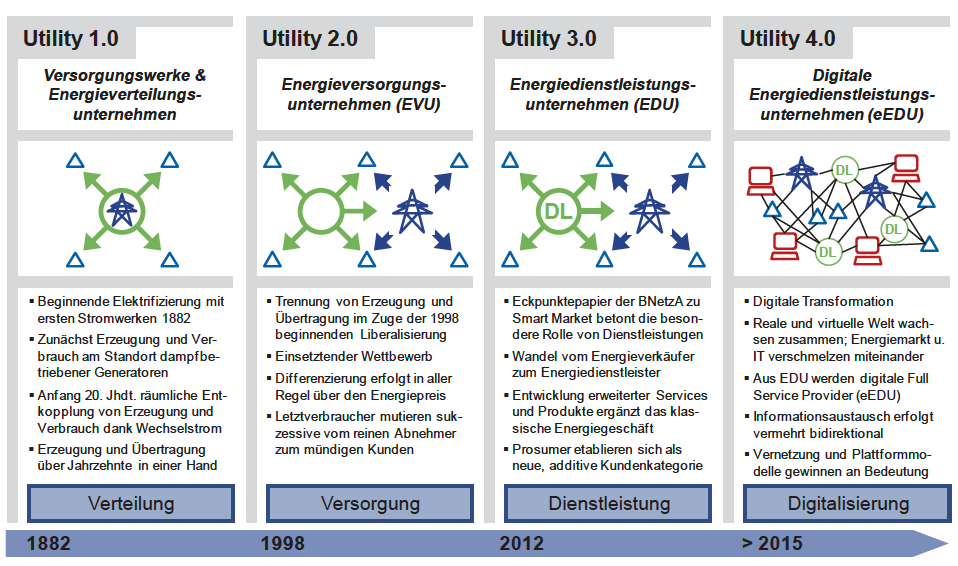
\includegraphics[width=1.0\linewidth]{utility_40.png}
  \caption[Transformation vom Versorgungswerk zum digitalen Energiedienstleister]{Transformation vom Versorgungswerk zum digitalen Energiedienstleister \citep[S. 13]{Doleski2016}}
\end{figure}

\begin{figure}[h]
  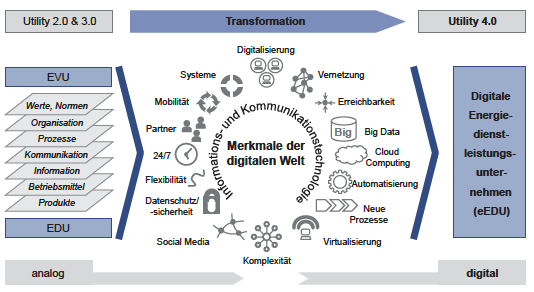
\includegraphics[width=1.0\linewidth]{kalalysator_utility_40.png}
  \caption[Digitale Welt als Katalysator für Utility 4.0 ]{Digitale Welt als Katalysator für Utility 4.0 \citep[S. 17]{Doleski2016}}
\end{figure}

Das Zusammenwachsen der pyhsischen und realen Welt zu mit Sensorik und Aktorik ausgestatteten Objekten, die mit dem Internet der Dinge miteinander vernetzt werden, erfordert eine Standardisierung \citep{BITKOM2015}.



Anforderung:Standardisierung


nach RAMI 4.0
RAMI (Referenzarchitekturmodell Industrie) 4.0: OPC-UA: Kommunikationsstandards (inkl. Sicherheit)
Sensorik: Bedeutung und sehr oberflächlich Funktionsweisen beschreiben
Gateways: Edge Processing
Device Management
Digital Twins

\subsection{Innovationsplattform}
Auch hierbei gilt das Prinzip des \textcolor{red}{Netzwerkeffekts} (s. 2.1.4): der Mehrwert besteht in der integrierten Anwendung in einem Kernsystem \citep{Elsner2018}.


Vorgedachtes Modell für Geräte (Thing Modell), IoT Services Anbindung Sensoren und Endgeräten, kalter, warmer, heißer Speicher
Best Practices and Design Thinking
\begin{itemize}
  \item Innovationsplattform ist nahtlos mit dem digitalen Kern (ERP) als Unternehmensgedächtnis \citep{Utecht2018} verbunden -> bimodale IT
  \item Einfache Anbindung an Backend Systeme
  \item z.B. ohne Materialstamm und Equipmentstamm kein Digitaler Zwlling
  \item Technologien IoT, Machine Learning, Blockchain, Analytics auch kurz beschreiben, was SAP da anbietet
  \item Auch eigene Leonardo-Produkte wie Connected Goods cloudbasierte IoT Anwendung, für Moni†oring von Produkten um ihren Wert zu maximieren wie Kühlketten, Verbräuche und Bestände
  \item SAP Connected Assets für Anlagegüter
\end{itemize}


\subsubsection{SCP}

Die Neo-Umgebung unterstützt hauptsächlich die Entwicklung von Java-Anwendungen sowie von nativen SAP HANA Anwendungen auf einem JavaScript Applikationsserver. Deren Benutzerschnittstellen können ausschließlich mit dem dem Frontend-Toolkit SAPUI5 entwickelt werden. Dafür steht in der Umgebung eine browserbasierte Entwicklungsumgebung, die SAP Web IDE, bereit.

Verschmelzung von IaaS und PaaS -> Einfacher, Services von Überall her zu nutzen





SAP Cloud Platform und AWS Microservices und APIs
Programmiersprachen und Laufzeitumgebungen
alle gängigen IaaS können zum deployen genutzt werden
Entwicklungsumgebung SAP Web IDE und Laufzeitumgebungen
CF, NEO, ABAP
Destinationsss
Innovationsplattform
Functional Services und Business Services
Cloud-to-Cloud Integration möglich (Elsner S.247) um Kompetenzen zu vereinen. z.B. Telekom Cloud mit SCP
Embedded Platform as a Service mit zwei Lösungsvarianten. SAP Cloud Platform - Neo Environment and SAP Cloud Platform - Cloud Foundry Environment
Datenbankservices wie verschiedene SAP-HANA-Versionen, MongoDB, PostgreSQL usw
Portalservices: Fiori Launchpad als Anwendungsportal
Application Runtime als Java-Anwendung oder XS-Anwendung Entwicklung mit WEB IDE
Konnektivitätsservice: SAP Cloud Platform Integration
\ac{api}

\begin{quotation}
  cf push - and your app is alive -> in die Systemanalyse
\end{quotation}


Leonardo erlaub die Wiederholung des Design Thinking Prozesses, da mit SCP und Microservice architekur easy skalierbar und anpassbar
Das Bild vielleicht eher in Umsetzungskonzept? oder in Vorgehen

\subsubsection{Use Case}
Weil das aktuelle \ac{scada}-System nur alle zehn Minuten Daten erfasst, soll es mit dem Ziel der Echtzeitfähigkeit auf eine Erweiterbarkeit mit SAP Technologien geprüft werden.

Ziel: Geschäftsfeld ändern und Echtzeitfähigkeit SCADA mit Leonardo über Kommunikationsschnittstellen

Neben der Datenerfassung und Fernüberwachung können Anlagen und Windparks aus der Ferne gesteuert und geregelt werden


 Obwohl viele ihrer Anlagen bereits Condistion Monitoring Systeme haben, gibt es noch immer Anlagen, die nicht internetfähig sind. Da das Ersetzen der Anlagen durch neue IoT-fähige Anlagen sowohl Ressourcenverschwendung als kostenspielig wäre, werden diese mit entsprechender Systemelektronik (Sensorik/Edge Geräte) nachgerüstet auch (s. retrofit). Diese Anlagen sollen digital abgebildet werden, um Zustände erfassen zu können. Nun fragt sich Enercon, vor allem im Zuge der Umstellung auf die von SAP HANA ermöglichten Im-Memory-Leistungen und weil die Stammdaten (Unternehmensgedächtnis, Basis für digital Twin) im SAP System liegen, wie sich wohl SAP Produkte für Monitoring und predictive maintenance eignen.
Außerdem verfolgen Sie zukünfig das Ziel, ihr Geschäftsfeld noch weiter zu erweitern, indem sie neben Produktion von Energie auch IT-Dienstleistungen z.B. für die Energieversorger im Zusammenhang mit den Produktionanlagen anzubieten.
Ich werde beauftragt, die Systemlanschaft von SAP Produkten (insb. Leonardo) für die digitale Transformation zu analysieren und prototypisch darstellen, wie/ob der Zustand einer (alte) WEA erfasst werden kann und ob auf Zustandsänderungen reagiert werden kann. Da Enercon ein global Player ist, möchten sie sich an RAMI 4.0 orientieren und die Informationssicht standardisiert haben. Auch das soll geprüft werden. Außerdem prüfen, wie die offlinefähigkeit ist und analysieren, welche Fähigkeiten das System zur Erweiterung des Industrie-4.0Netzes bietet.
